\documentclass{article}
\usepackage{amsmath, amssymb}
\usepackage[letterpaper, margin=1in]{geometry}
\usepackage{graphicx}
\usepackage{authblk}
\usepackage{float}
\usepackage{libertine}
\usepackage[libertine]{newtxmath}

\DeclareMathOperator*{\argmax}{argmax}

\title{Project 2 --- Face and Digit Classification}
\author{Fernando Gonzalez}
\author{Pranav Prakash}
\author{Wanyun Liu}
\affil{\textit {\{fdg17, pp618, wl432\}@scarletmail.rutgers.edu}}
\date{\today}

\begin{document}
  \maketitle
  \section{Classification Algorithms}
  \subsection{Naive Bayes}
  Our goal in using the Naive Bayes classifier is to compute the probability that a given image has a certain label,
  given that a set of features is observed. 
  The Naive Bayes algorithm classifies images by keeping track of two sets of data.
  To discover what these sets of data should be, we first introduce Bayes' Rule:
  \begin{equation}
  \Pr(A \mid B) = \frac{\Pr(B \mid A)\Pr(A)}{\Pr(B)}
  \end{equation}
  Since we want {\em the probability that} an image has a certain label, {\em given that} we observe it has a certain set of features,
  we should let $A$ refer to the label or {\em class}, and $B$ to a set of features. 
  The image classes are the set of all labels that can be given to an image.
  When classifying digits, these are the actual digits $\{0, 1, \ldots, 9\}$.
  For faces, the classes are {\em `not-face'} and {\em `face'},
  where {\em `not-face'} is represented by 0 or False, and {\em `face'} is represented by 1 or True.
  We let $Y, y$ refer to classes, and $X, x$ refer to features, where capitals are random variables. $N$ is the total number of features in an image.
  \begin{equation}
  \Pr(Y = y \mid \bigcap_i^NX_i = x_i) = \frac{\Pr(\bigcap_i^NX_i = x_i \mid Y = y)\Pr(Y = y)}{\Pr(\bigcap_i^NX_i = x_i)}
  \end{equation}
  First are the {\em prior probabilities}, which are estimated by:
  \begin{equation}
  \text{Prior}(y) = \Pr(Y = y) = \frac{\text{number of images with label = y}}{\text{total number of images}}
  \end{equation}
  Observing from (2) that $\Pr(Y = y)$ is the prior probability $\text{Prior}(y)$, and assuming the feature probabilities are conditionally independent, we have:
  \begin{equation}
  \Pr(Y = y \mid \bigcap_i^NX_i = x_i) = \frac{\Pi_i^N\Pr(X_i = x_i \mid Y = y) \cdot \text{Prior}(y)}{\Pr(\bigcap_i^NX_i = x_i)}
  \end{equation}
  By looking for the class which maximizes this value, we can simplify this further to get our final equation:
  \begin{align}
  \argmax_y (\Pr(Y = y \mid \bigcap_i^NX_i = x_i)) &= \argmax_y( \Pi_i^N\Pr(X_i = x_i \mid Y = y) \cdot \text{Prior}(y)) \\
  &= \argmax_y \log (\text{Prior}(y) \cdot \Pi_i^N\Pr(X_i = x_i \mid Y = y)) \\
  &= \argmax_y (\log \text{Prior}(y) + \log \sum_i^N\text{Cond}(i, x_i, y))
  \end{align}
  As stated previously, Prior$(y)$ is computed by finding the proportion of images with label $y$ compared to the total number of images.
  Cond$(i, x_i, y)$, the estimated probability that the feature at index $i$ has value $x_i$, given the label $y$, is given by:
  \begin{equation}
  \text{Cond}(i, x_i, y) = \frac{\text{number of times feature $i = x_i$ when label $= y$}}{\text{number of images where label $= y$}}
  \end{equation}
  The Naive Bayes classifier also has a Laplace smoothing parameter $k$, so that Cond$(i, x_i, y) \ne 0$, and to avoid direct usage of raw estimates, which could cause overfitting of the model to the training set.
  Our final equation for Cond, which we use to compute the {\em conditional probabilities}, is:
  \begin{equation}
  \text{Cond}(i, x_i, y, k) = \frac{k + \text{number of times feature }i = x_i \text{when label}= y}{(\text{number of classes}\cdot k) + \text{number of images where label}= y}
  \end{equation}
  The training period of the Naive Bayes classifier consists of computing Prior$(y)$ and Cond$(i, x_i, y, k)$ for all classes $y$, all pixel indices $i$, and all possible feature values $x_i$.
  This state is then used to classify images. The result of classification is the output of (7).
  \subsection{Perceptron}
  The Perceptron algorithm keeps track of a set of weight vectors $\vec{w}_{\,y}$.
  The weight vectors are indexed by class, so there is exactly one vector per class.
  The size of each vector is equal to the number of features in an image.
  For our purposes, this is the number of pixels in an image.
  These weight vectors can be initialized to any value, so we have initialized them with random values.
  The algorithm computes a guess by computing the dot product of each weight vector by the feature vector and selecting the class whose vector had the largest dot product: 
  \begin{align*}
  \text{score}(y) &= \vec{w}_{\,y} \cdot \vec{f}_{\,y} \\
  \text{guess}(y) &= \argmax_y \text{score}(y)
  \end{align*}
  With normalized vectors, the dot product of two vectors attains a maximum value (1) when the vectors are parallel (in this case, identical), and a minimum value (-1) when they are antiparallel (opposites).
  The ordering of this relationship remains true with non-normalized vectors (although the actual maximum and minimum will depend on the length of both vectors), so the dot product of the weight and feature vectors are a measure of their similarity.
  This is why we select the vector whose dot product with the actual feature vector is largest.
  If the guess is correct, nothing happens. Otherwise, the feature vector is added to the weight vector corresponding to the same class, and subtracted from the weight vector corresponding to the guess class:
  Letting $g$ refer to the label of the guessed class, we have:
  \begin{align*}
  \vec{w}_{\,y}  &= \vec{w}_{\,y} + \vec{f}_{\,y} \\
  \vec{w}_{\,g}  &= \vec{w}_{\,g} - \vec{f}_{\,y} 
  \end{align*}
  \section{Implementation}
  \subsection{Features}
  Pixels were directly extracted to ternary features: 0 for an empty pixel, 1 for a `grey' pixel (represented by `+'), and 2 for a `black' pixel (represented by `\#').
  These were directly used in the case of the Perceptron algorithm, but for the Naive Bayes algorithm, the features were mapped to indicator triples $[f(X_i), g(X_i), h(X_i)]$,
  where $f(X_i) = 1$ if $X_i = 0$, $g(X_i) = 1$ if $X_i = 1$, $h(x_i) = 1$ if $X_i = 2$, and zero otherwise.
  \subsection{Parameters}
  \paragraph{Naive Bayes}
  Naive Bayes uses Laplace smoothing to improve accuracy and reduce overfitting. We used a constant value of 2 for the Laplace smoothing constant.
  \paragraph{Perceptron}
  The number of times the training data is iterated over can be customized under Perceptron. 
  Note that a higher number of iterations is not necessarily better due to the possibility of overfitting.
  We used a constant value of 5 for the number of iterations.
  \subsection{Results}
  Results were calculated by iterating over each algorithm 25 times for each data point.
  The accuracy, standard deviation, and timing data were averaged over these 25 iterations to produce the data points represented in the graphs below.
  \subsubsection{Digit Classification}
  \paragraph{Accuracy}
  \begin{figure}[H]
  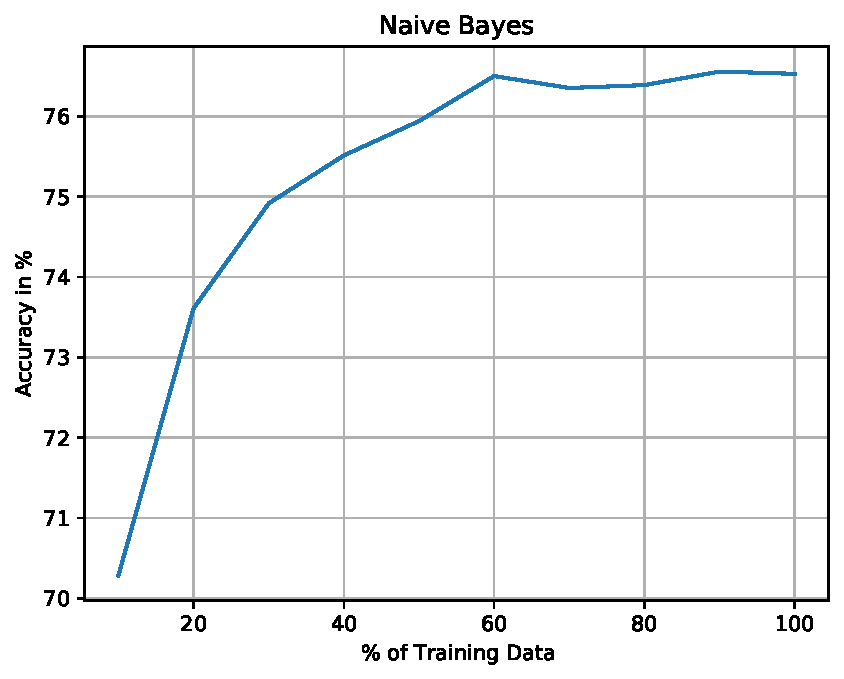
\includegraphics[width=0.45\linewidth]{figures/Naive Bayes_accuracy_DIGIT.pdf}\hfill
  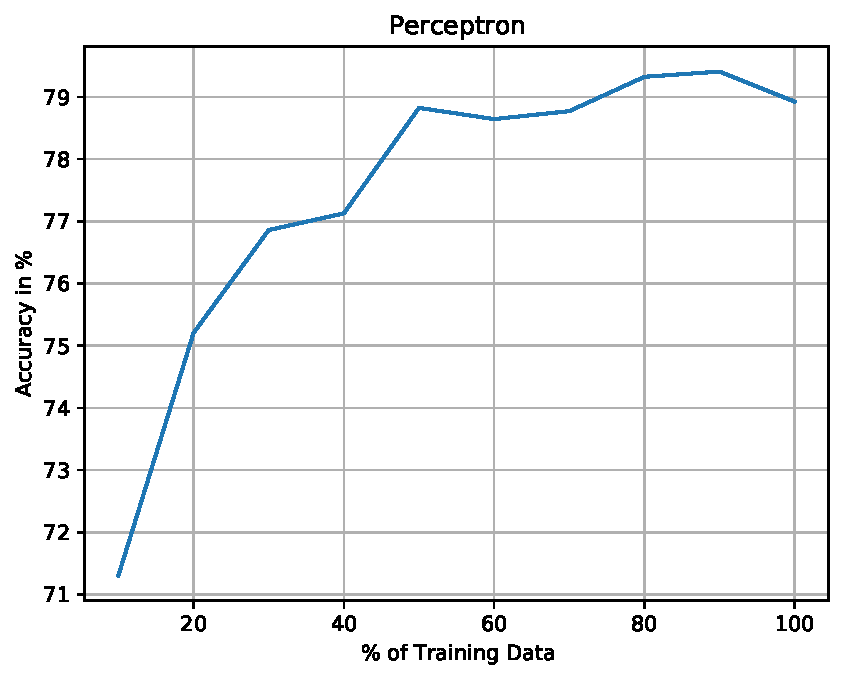
\includegraphics[width=0.45\linewidth]{figures/Perceptron_accuracy_DIGIT.pdf}\hfill
  \caption{Accuracy for Digit Classification}
  \end{figure}
  As we can see, the accuracy for both algorithms in terms of the training data behaves like $sqrt(x)$.
  However, note that the Perceptron accuracy data is more erratic.
  The accuracy of Perceptron is slightly higher than that of Naive Bayes, but it is still strictly better than Naive Bayes at each data point.
  \paragraph{Standard Deviation}
  \begin{figure}[H]
  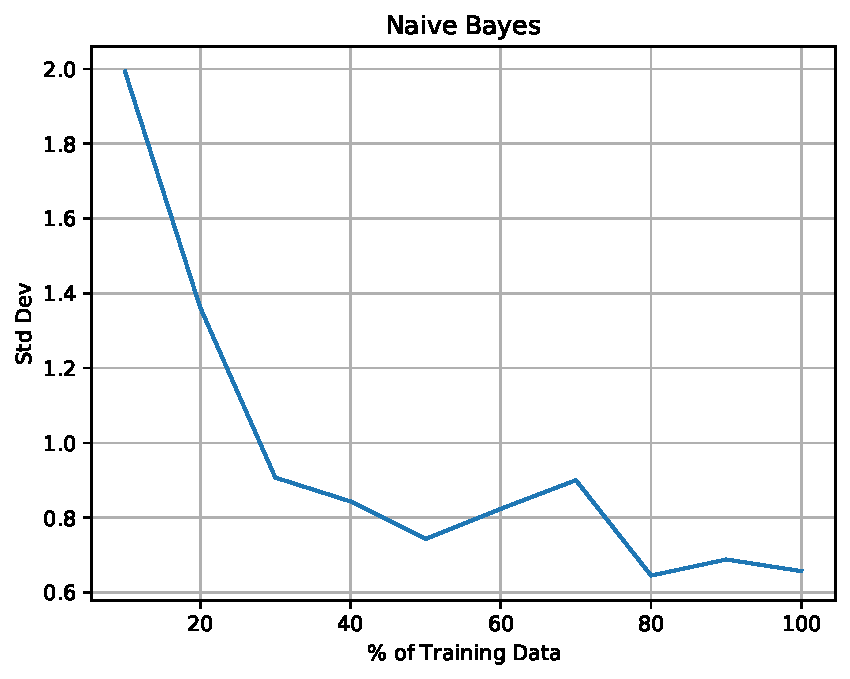
\includegraphics[width=0.45\linewidth]{figures/Naive Bayes_stddev_DIGIT.pdf}\hfill
  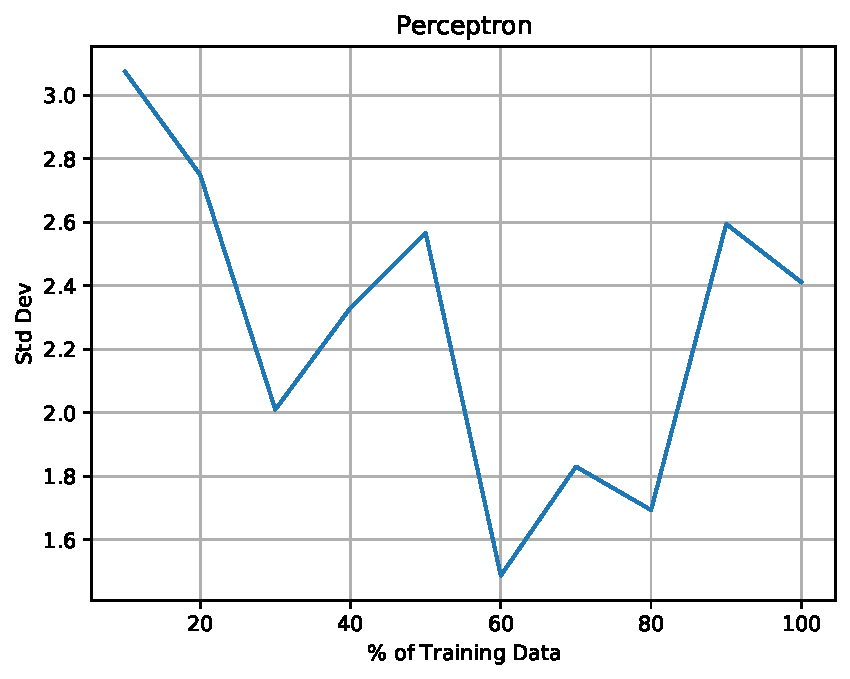
\includegraphics[width=0.45\linewidth]{figures/Perceptron_stddev_DIGIT.pdf}\hfill
  \caption{Standard Deviation for Digit Classification}
  \end{figure}
  When it comes to the standard deviation in Naive Bayes, we see it fluctuating in the lower percentages of training data and then somewhat steadily decreasing after around 50\%. 
  This is expected due to the sparseness of the training data at low percentages.
  The Perceptron data trends downwards but again fluctuates much more violently. 
  The range for the standard deviations of both algorithms is about the same (1.4), however Perceptron is about one standard deviation higher at all times.
  This variance does not appear to be caused by underfitting and overfitting, as we observe the same variance with the MNIST database.
  It is also interesting to note that low standard deviations roughly correspond to high accuracy values.
  This allows us to conclude that the Naive Bayes algorithm is much more stable (lower variance), while the Perceptron algorithm is more accurate but much less stable (higher variance).
  \paragraph{Training Time}
  \begin{figure}[H]
  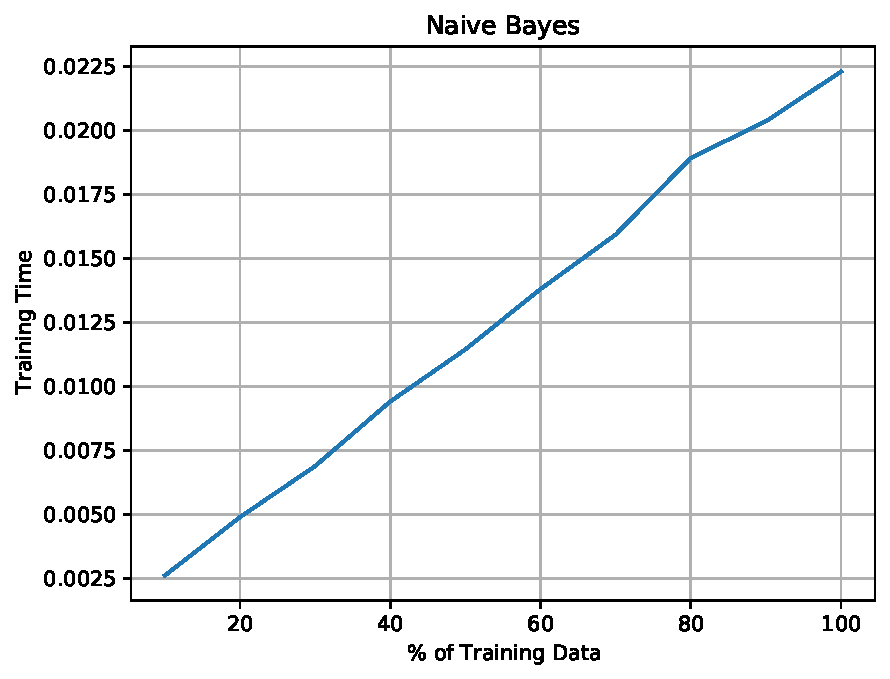
\includegraphics[width=0.45\linewidth]{figures/Naive Bayes_time_DIGIT.pdf}\hfill
  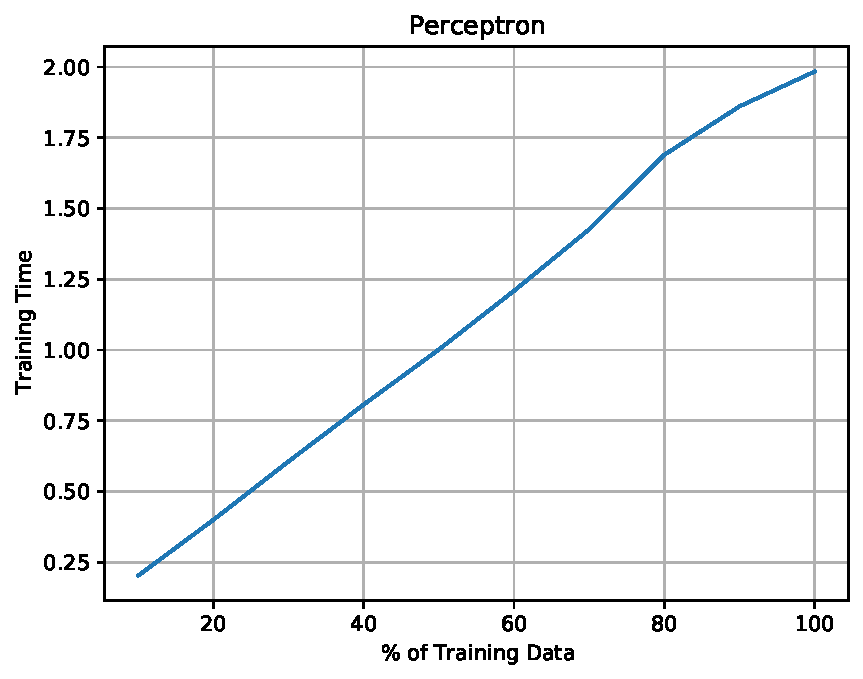
\includegraphics[width=0.45\linewidth]{figures/Perceptron_time_DIGIT.pdf}\hfill
  \caption{Training Time for Digit Classification}
  \end{figure}
  The training time for both algorithms show a clear linear trend.
  The training time for Perceptron is much higher than Naive Bayes. 
  However, note that the training time for Naive Bayes is extremely low, never reaching higher than 30 milliseconds.
  It is entirely possible that Naive Bayes is faster only because it is much more heavily optimized.
  The Perceptron algorithm uses almost pure linear algebra, making it a good candidate to take advantage of vectorization, so it is quite possible that the Perceptron classifier could stand to be much more optimized.
  \subsubsection{Face Classification}
  The trends are similar to the digit data but have been added in for the sake of completeness. 
  We see that the accuracy curve for Perceptron is smoother here. 
  One thing to note is that the training times for both algorithms are substantially lower here, which is expected since there are only two classes, instead of the ten classes for digit classification.
  There are also less training images than for digit classification and the images are much smaller.
  For this reason, we observe much higher standard deviations and much lower starting accuracies.
  Note, however, that while Naive Bayes starts at a pitiful 55\%, Perceptron gets about 71\% accuracy with only 10\% of training data, before performing about the same near 100\% of training data.
  \begin{figure}[H]
  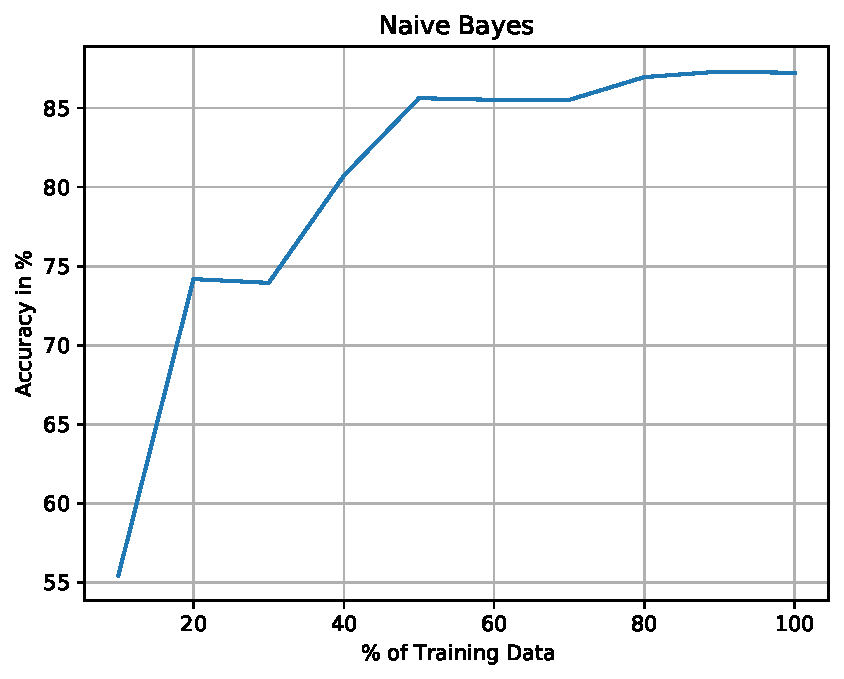
\includegraphics[width=0.45\linewidth]{figures/Naive Bayes_accuracy_FACE.pdf}\hfill
  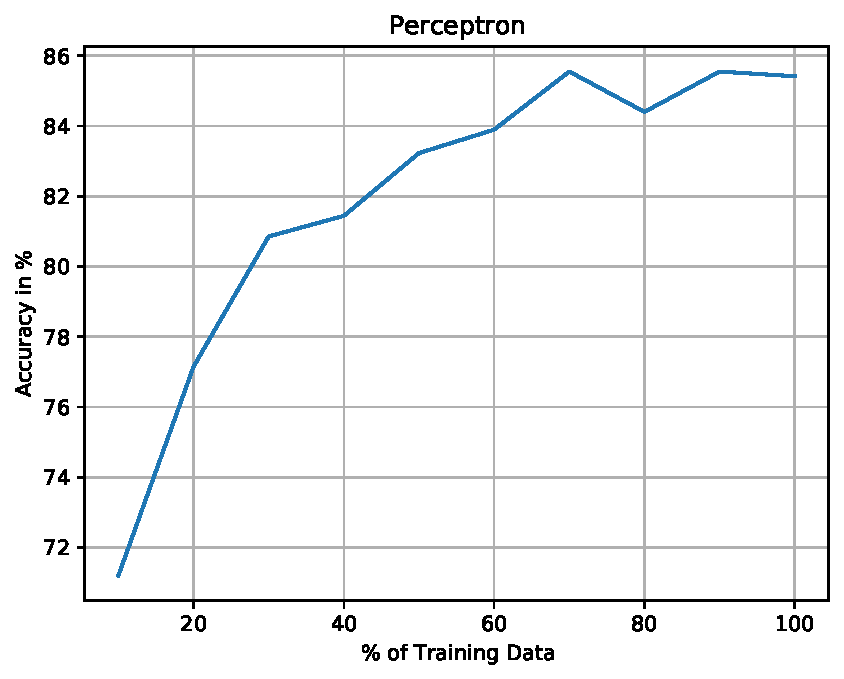
\includegraphics[width=0.45\linewidth]{figures/Perceptron_accuracy_FACE.pdf}\hfill
  \caption{Accuracy for Face Classification}
  \end{figure}
  \begin{figure}[H]
  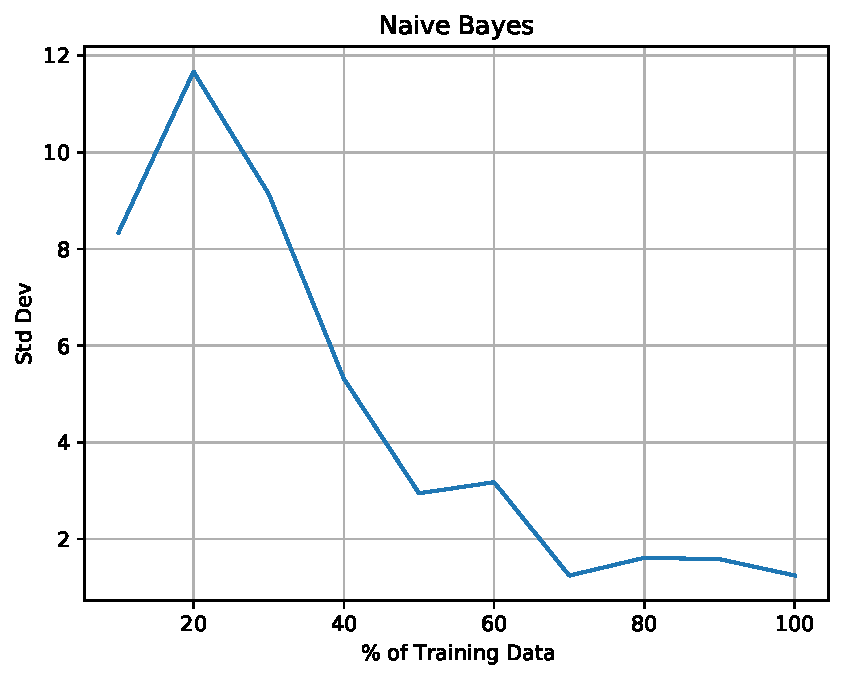
\includegraphics[width=0.45\linewidth]{figures/Naive Bayes_stddev_FACE.pdf}\hfill
  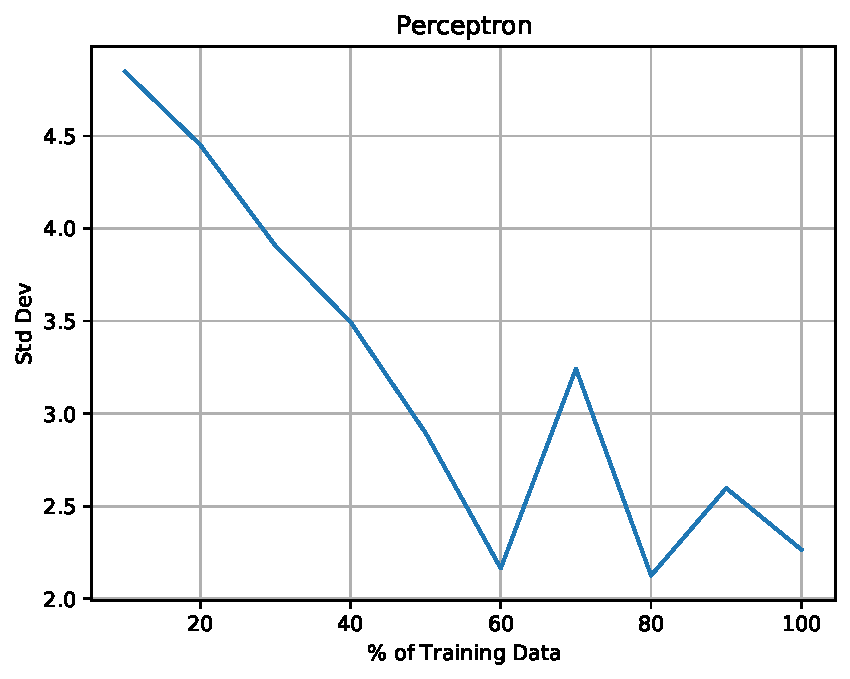
\includegraphics[width=0.45\linewidth]{figures/Perceptron_stddev_FACE.pdf}\hfill
  \caption{Standard Deviation for Face Classification}
  \end{figure}
  \begin{figure}[H]
  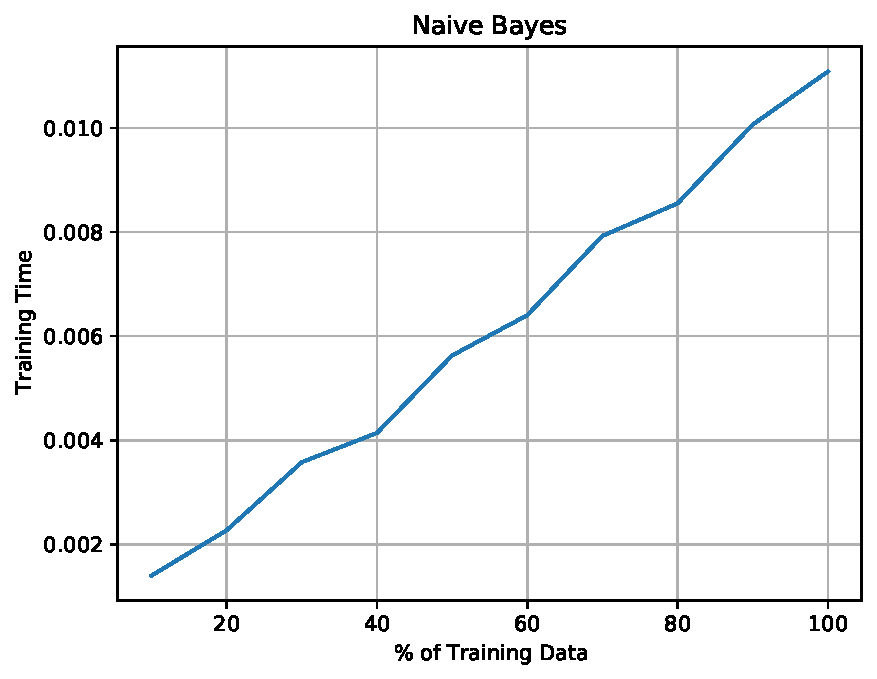
\includegraphics[width=0.45\linewidth]{figures/Naive Bayes_time_FACE.pdf}\hfill
  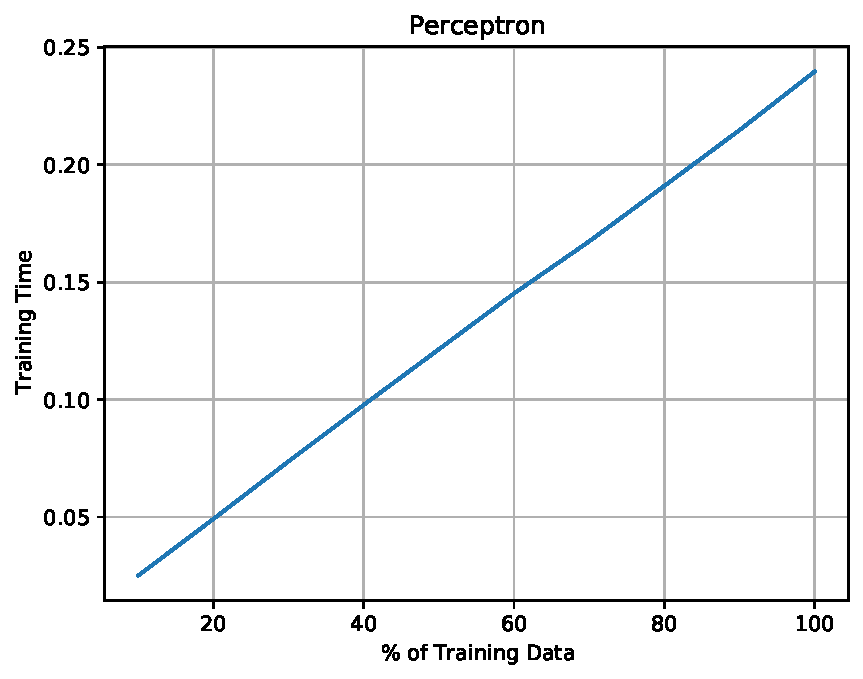
\includegraphics[width=0.45\linewidth]{figures/Perceptron_time_FACE.pdf}\hfill
  \caption{Training Time for Face Classification}
  \end{figure}
  \subsubsection{MNIST}
  \begin{figure}[H]
  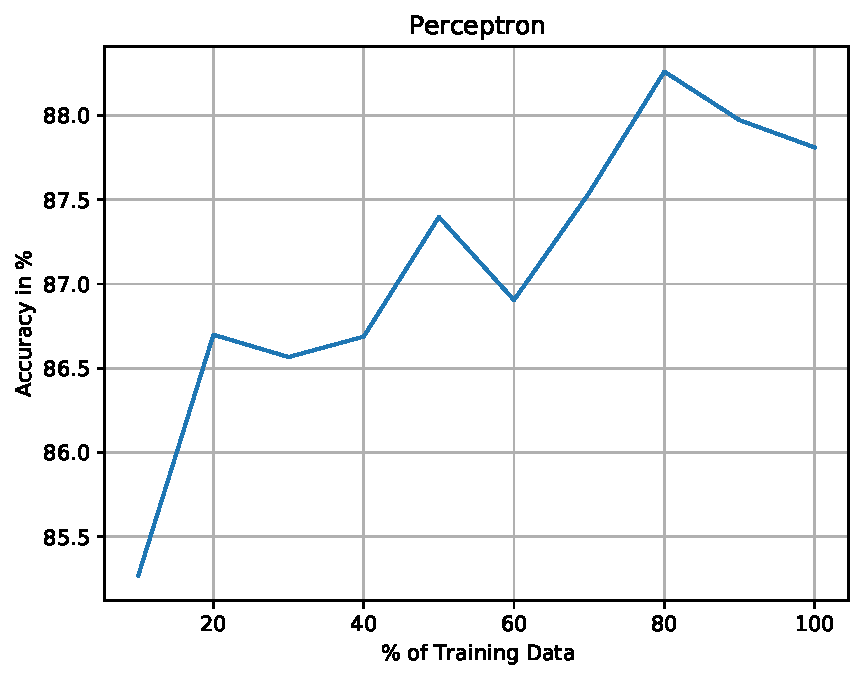
\includegraphics[width=\linewidth]{figures/Perceptron_accuracy_MNIST.pdf}\hfill
  \caption{MNIST Classification -- Accuracy}
  \end{figure}
  \paragraph{Accuracy}
  Here, we test the Perceptron classifier against the openly available MNIST database, which has 60000 training images and 10000 test images of handwritten digits.
  It is very interesting to note that our Perceptron algorithm has an accuracy of around 85\% with only 10\% of the training data. :)
  This is likely because the MNIST database is extremely large, and so 10\% of the training data is still 6000 images.
  Interestingly, we still observe the high variance in accuracy found in the digit classification data.
  This data appears to confirm the hypothesis that the variance found in the accuracy data is related to instability inherent to the Perceptron algorithm, rather than an implementation quirk or error.
  \begin{figure}[H]
  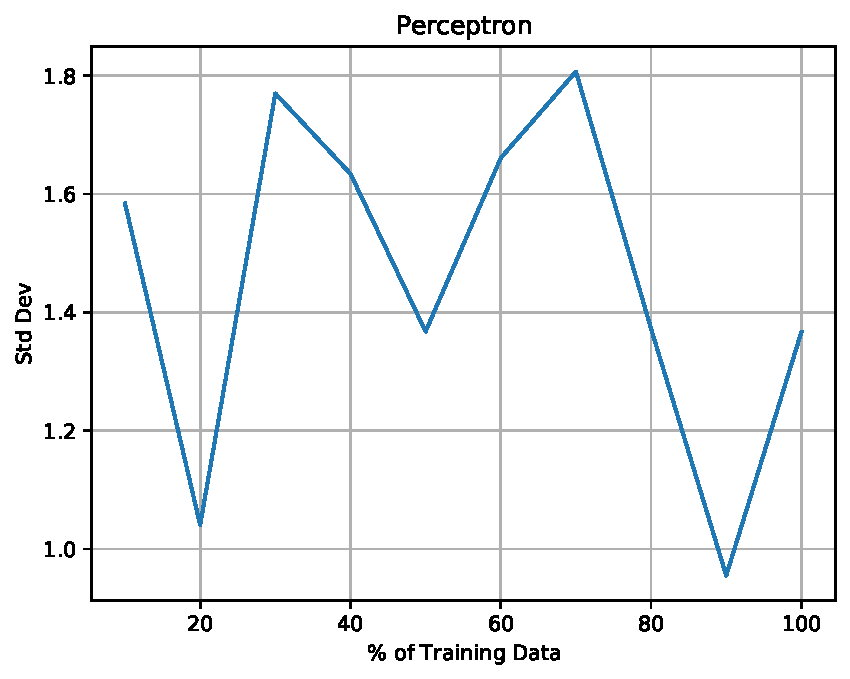
\includegraphics[width=\linewidth]{figures/Perceptron_stddev_MNIST.pdf}\hfill
  \caption{MNIST Classification -- Standard Deviation}
  \end{figure}
  \paragraph{Standard Deviation}
  While the graph appears erratic, the standard deviation in MNIST classification is bounded by 0.9 and 1.9, so it has a total range of about 1.
  Standard deviation appears to have almost no correlation with percentage of training data.
  We continue to observe that spikes of standard deviation correlate with low accuracy, and vice versa.
  \begin{figure}[H]
  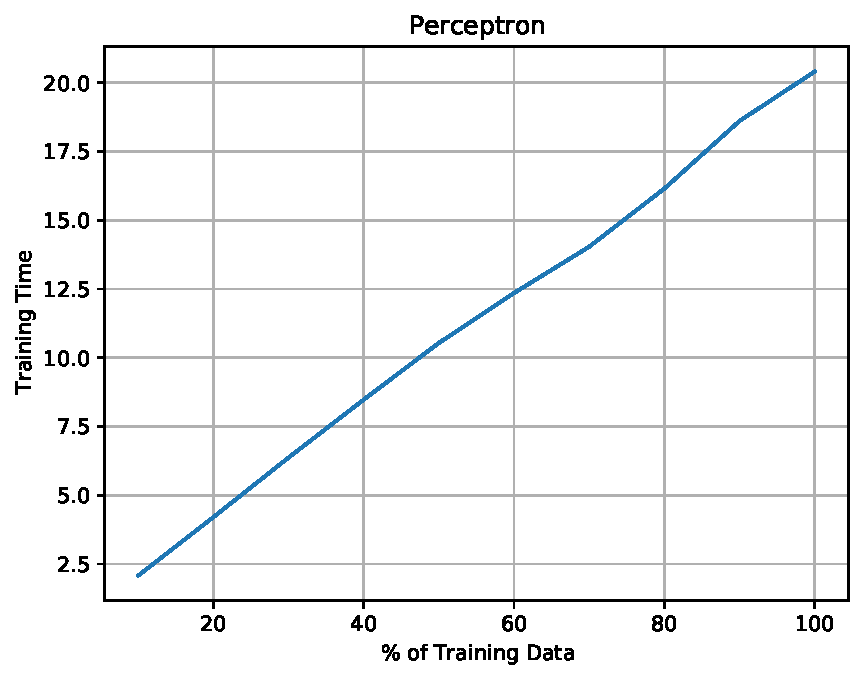
\includegraphics[width=\linewidth]{figures/Perceptron_time_MNIST.pdf}\hfill
  \caption{MNIST Classification -- Training Time}
  \end{figure}
  \paragraph{Training Time}
  As a sanity check, the MNIST training time data reveals a remarkably linear trend.
  Please note the painful running time of 20 seconds per iteration at 100\% training data.
  Data points were computed by averaging the running time of 25 iterations, for all ten data points, for a total 250 iterations.
  At 100\% training data, the last 25 iterations would have taken (read: {\em took}) about 500 seconds to complete, or 8 minutes and 20 seconds.
  It is almost certain that our implementation of Perceptron can be further optimized.
  \paragraph{Naive Bayes}
  In order to adapt MNIST image data to work with Naive Bayes, it would have been necessary to expand each feature into an indicator vector with 256 entries, as MNIST pixels can have any value from 0 to 255.
  This proved infeasible, and would have to be done in a very clever fashion to prevent explosion of time and space complexity.
  For this reason, MNIST classification using the Naive Bayes algorithm was not implemented.
  \subsection{Obstacles}
  \paragraph{Core Logic}
  The logic of the algorithms was straightforward.
  Implementation of Naive Bayes was a minor issue due to optimization, but overall, implementation of the core logic of the algorithms themselves was not much of an issue.
  Perceptron is even simpler than Naive Bayes, so implementation was not an issue at all.
  \paragraph{Optimization}
  The biggest task was optimization of our initial implementations to get the runtime down to an acceptable level.
  The \texttt{numpy} library was instrumental in massively reducing runtimes.
  This is because of the builtin vectorization that \texttt{numpy} uses throughout its operations to compute large amounts of linear operations simultaneously.
  Machine learning algorithms often heavily rely on vectorization due to the fact that they are very intensive on linear algebra operations.
  In the case of Perceptron, the algorithm is almost pure linear algebra, as guesses are computed via dot products, and adjustments are component-wise vector sums.
  Because of this, basically all of the Perceptron algorithm can be vectorized.
  \paragraph{Data Structuring}
  For Naive Bayes, similar optimizations could be taken advantage of through clever use and shaping of data via \texttt{numpy}.
  This is why features were represented as `indicator vectors' for Naive Bayes: grouping the images together by label and computing a sum along the axis of images automatically counted the number of times a given pixel had a given feature, and in a vectorized fashion.
  The sum would transform the large array of features into a 10x784x3 array, where e.g. $counts[4, 100, 2]$ held a value equal to the number of times the pixel at index 101 had the feature 2 in all images labeled as 4.
  These counts were computed in one line using \texttt{numpy}, so the computation is highly parallelized due to \texttt{numpy}'s vectorization.
  For this reason, the training time for Naive Bayes never exceeded {\em 30 milliseconds}.
  It is likely that the Perceptron running time is so much higher than Naive Bayes because of how heavily optimized the Naive Bayes classifier was.
  In general, machine learning algorithms appear to be highly parallelizable, so proper structuring of data and use of vectorization is essential for performant algorithms.
\end{document}
